\section{Introduction}
The application-based IoT system used in this project involves 4 main layers of the standard IoT environment. The abstract view of the system is depicted in Figure \ref{fig:iot-system}, in which the 4 main modules are highlighted in 4 different colors and the communication protocols between them are also included as interconnecting arrows. Communication involves both wireless protocols (depicted as dash arrows) and wired connections (depicted as normal arrows). The names of the communication protocol being used are typed right beside the corresponding arrows. We only have 2 communication protocol in this project: MQTT protocol and UART communication. The implementation of these protocols will further be explain in more detail later.
\begin{figure}
    \centering
    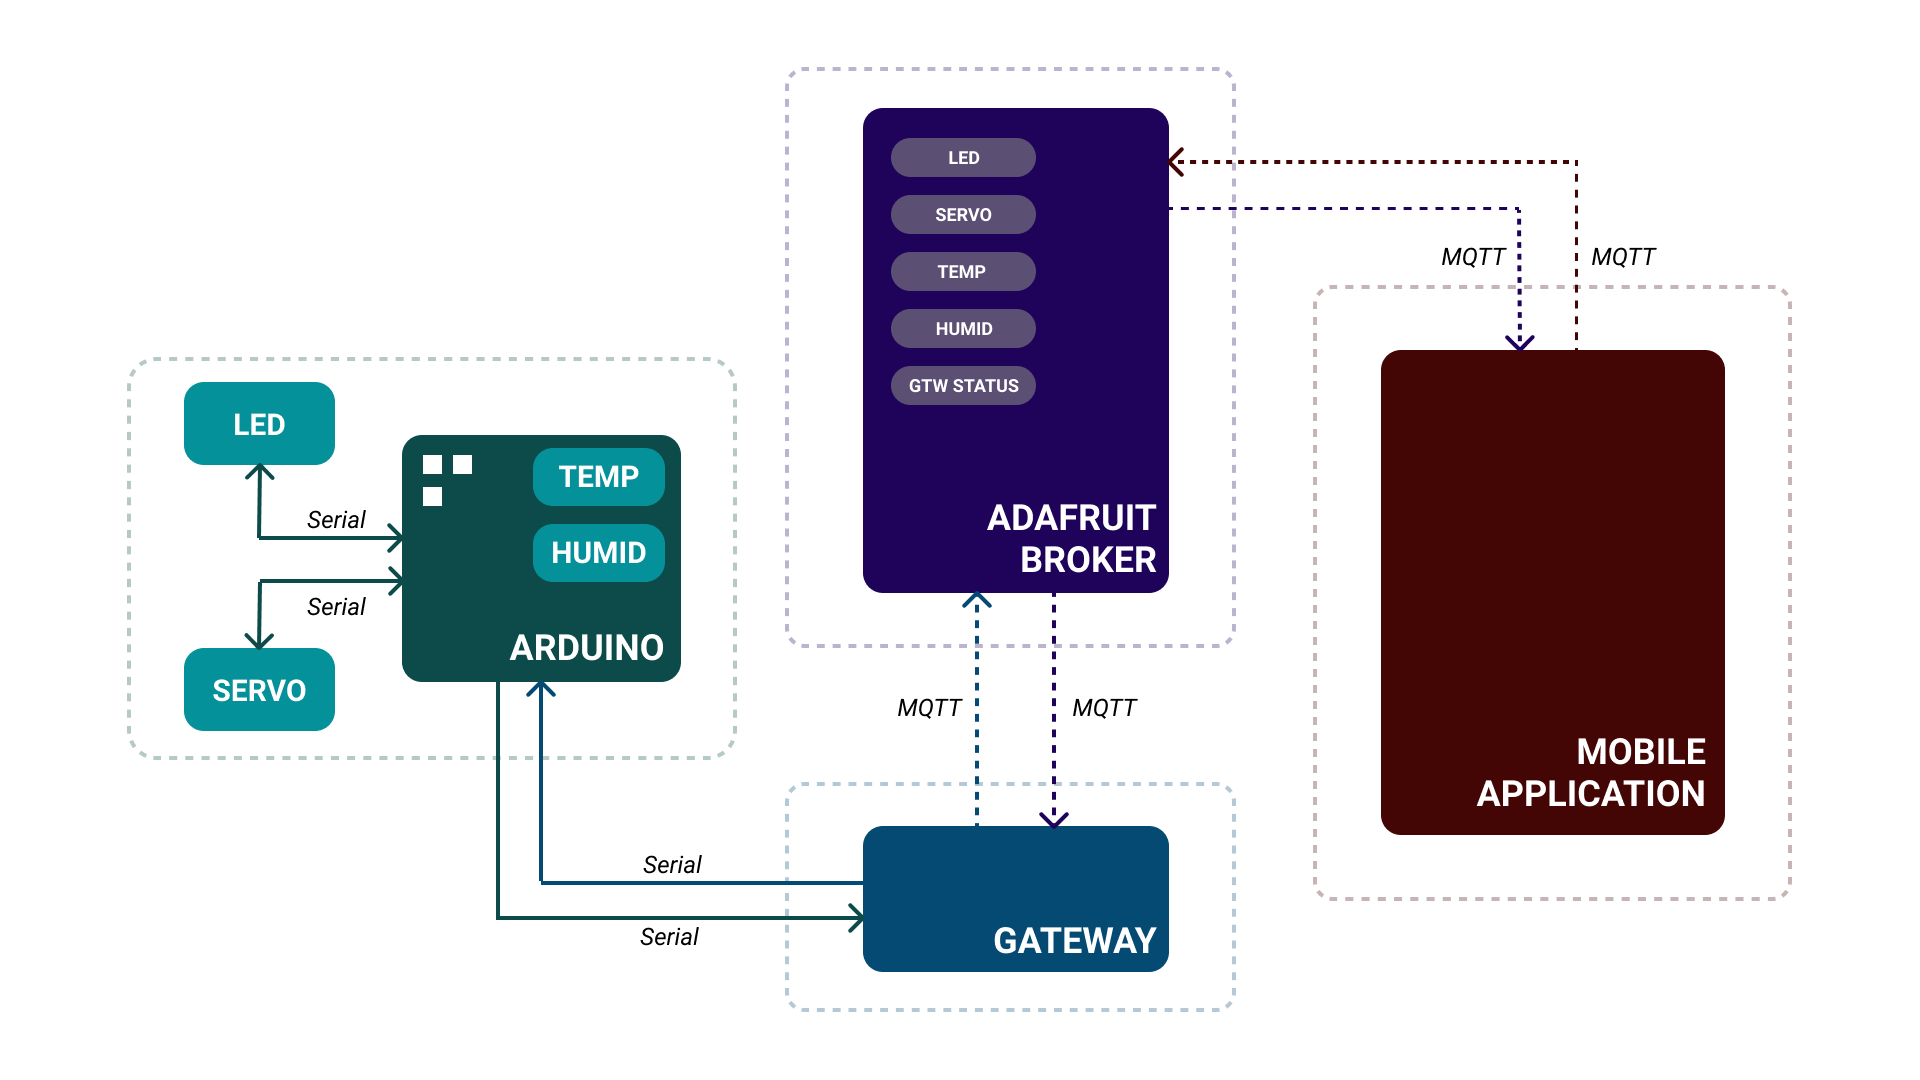
\includegraphics[scale=0.25]{graphics/Overall Architecture.png}
    \caption{IoT System Layers}
    \label{fig:iot-system}
\end{figure}

The first module of our system is the \textbf{Arduino Node}. This layer of the IoT system do the simple assembly work that receives data from the external \textit{Led} and \textit{Servo} device, as well as generates random \textit{Temperature} and \textit{Humidity} value. The \textit{Arduino} is also responsible for sending these data packets through UART communication to the next module, the Gateway layer.

Acting as an intermediate module, the \textbf{Gateway} constantly monitors the incoming data packets from both the Arduino and the Adafruit Broker. Its main job is to handle these data and dispatch (send) them to the correct destination. An additional and important feature of the Gateway is to fetch the latest data from the broker and send them to the Arduino node when it first connect (or reconnect) to the server. The implementation of the Gateway will also be explained in more detail in later part of the document.

The broker used in this project is the service provided by the \textbf{Adafruit IO} cloud. The broker provides enough \href{https://io.adafruit.com/api/docs/mqtt.html#adafruit-io-mqtt-api}{\textcolor{blue}{API implementation}} for MQTTv3.1 standard. Our IoT system will have 5 separate feeds on the server to record and distribute data to any client connecting to the broker. We have the \textit{Gateway} is the first MQTT client by which we publish data packets from the \textit{Arduino Node} to the online feeds. Gateway client also subscribes to several (but not all) necessary topics from the broker to receive request messages from the server. The broker maintains an additional feed called \texttt{gtw-status} that record the current status (\textit{online}/\textit{offline}) of the Gateway. Whenever our Gateway successfully connects to the broker, it will automatically set its status to \textit{online} by publish a short message to this feed. In the event the Gateway is \textbf{willing} to disconnect from the server, it will publish an \textit{offline} message to the status topic before leaving. This will be further explained when we come to the implementation of the Gateway.

The second MQTT client, also the last layer of out IoT system, is the \textbf{mobile application}  module. It is at this layer the users have a decent interface to monitor and interact with the IoT components. Much like the Gateway, our mobile application implements the v3.1 version of the MQTT protocol to communicate with the Adafruit server. The detail of the mobile layer is saved until we come to the section \ref{mobile-application}.

Now that's the overview to the IoT architecture. We now continue to explore how to actually put these modules down in the upcoming sections. Before going on, in order to ease up tracking the implementation, the whole project can be found at this Github \href{https://github.com/hescul/adafruit-simple-iot}{\textcolor{blue}{repository}} hosted by the author of this document.
\clearpage